\chapter{Porting Tang}\label{porting-tang}

After successfull cross-compilation of jose we have all the dependencies "ready" and packaged except the systemd.
We need to configure socket activation because Tang is not implemented to create its own sockets.


\section{Socket activation}

Socket activation is a technology provided by a super-server or sometimes called a service dispatcher daemon.
A super-server starts other servers when needed as well, normally with access to them checked by a TCP wrapper.
It uses very few resources when in idle state.

systemd is only one of the many implementations (inetd, launchd, ucspi-tcp, xinetd) of a super-server providing socket activation.



\subsection{xinetd}
xinetd offers a more secure alternative to the older inetd ("the Internet daemon"), which most modern Linux distributions have deprecated.
Without socket activation a service designed for it is behaving as CLI application with input read from stdin and output written to stdout.
The socket activation service is listening on assigned port.
It creates the socket when the request and spawn an application instance with redirecting stdin and stdout to the socket created.
\begin{figure}[h]
    \centering
    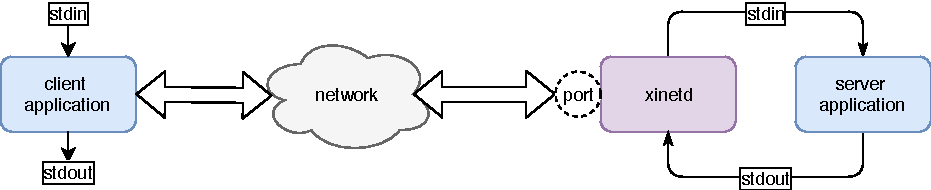
\includegraphics[scale=0.9]{figures/xinetd.pdf}
    \caption{xinetd socket activation}
    \label{fig_xinetd}
\end{figure}
xinetd is supported by and packaged for OpenWrt already.
\section{Install dependencies}

As we have all of the Tang dependencies "ready"

update feeds
feeds install
make menuconfig
\newpage



to have an example created simple application in C for xinetd
\newpage

\section{Cross-compile Tang}

do not forget to add xinetd in Dependencies
\newpage

\subsection{Hurdles with http-parser}\label{http_parser_problems}

without upstream patch not working tang
\newpage

\subsection{Mysterious José}

does makefiles support shell {a,b} thing???
\newpage

\section{Configure Tang with xinetd}

We need xinetd's socket activation for Tang to work.


there is no systemd for OpenWrt

/etc/services

xinetd configuration

\subsection{}


% root@A04-0315A:~# if [ -z "$(find /usr/share/tang/db/ -name "*.jw*" -maxdepth 1)" ]; then echo nic; else echo daco;fi
% daco
% root@A04-0315A:~# if [ -z "$(find /usr/share/tang/db/ -name "*.jwk" -maxdepth 1)" ]; then echo nic; else echo daco;fi
% daco
